\section{Dataset and Exploratory Analysis}
\label{sec:dataset_eda}

\subsection{The C-MAPSS Data Set}
We use the NASA C-MAPSS turbofan degradation data~\cite{Saxena2008turbofan},
generated with the simulator and damage-propagation model of Saxena
et al.~\cite{Saxena2008damage}. It has four subsets that differ in the number of
operating conditions and fault modes (Table~\ref{tab:subsets}). Every subset
has a training file, in which each engine is observed from an unknown initial
wear level until failure, and a test file, in which each trajectory stops at
some point before failure. A separate file gives the true RUL at the last
recorded cycle of each test engine. Engine identifiers are local to each
subset and split. FD001 is the primary subset of this project; the other three
show how the difficulty grows when operating conditions and fault modes are
mixed, which Ramasso and Saxena~\cite{Ramasso2014performance} identify as the
main obstacles to comparing results on this benchmark.

\begin{table}[!t]
\centering
\caption{C-MAPSS subsets. Engine and row counts are taken from the raw files;
lifetimes are the final cycles of the training engines.}
\label{tab:subsets}
\begin{tabular}{lcccccc}
\hline
Subset & Cond. & Faults & \multicolumn{2}{c}{Engines} & \multicolumn{2}{c}{Lifetime} \\
       &       &        & Train & Test & Median & Range \\
\hline
FD001 & 1 & 1 & 100 & 100 & 199   & 128--362 \\
FD002 & 6 & 1 & 260 & 259 & 199   & 128--378 \\
FD003 & 1 & 2 & 100 & 100 & 220.5 & 145--525 \\
FD004 & 6 & 2 & 249 & 248 & 234   & 128--543 \\
\hline
\end{tabular}
\end{table}

The fault mode is degradation of the high-pressure compressor (HPC) in FD001
and FD002; FD003 and FD004 add fan degradation. FD001 contains 20,631 training
rows and 13,096 test rows. Each row is one engine cycle with 26 columns: engine
identifier \texttt{unit}, cycle index \texttt{cycle}, three operating settings
\texttt{op\_1}--\texttt{op\_3} (altitude, Mach number and throttle resolver
angle) and 21 sensor channels $s_1,\dots,s_{21}$. The sensors record
temperatures, pressures, shaft speeds, ratios and bleed flows at different
engine stations; for example $s_2$, $s_3$ and $s_4$ are commonly identified
with the LPC, HPC and LPT outlet temperatures and $s_{11}$ with the HPC outlet
static pressure~\cite{Saxena2008damage}. RUL is not one of the columns. The
training target is the engine's final cycle minus the current cycle, and test
engines are scored only at their last observed cycle against the supplied RUL.

\subsection{Exploratory Findings}
The analysis below uses training trajectories only, so that no test
information shapes later modelling choices. It describes the data; the
transforms it motivates are fitted inside each training fold, as described in
Section~\ref{sec:feature_engineering}.

\subsubsection{Lifetimes differ widely between engines}
Fig.~\ref{fig:eda_lifetimes} shows that FD001 lifetimes range from 128 to 362
cycles around a median of 199, and the two-fault subsets are longer and more
spread out, reaching 525 and 543 cycles. Because an engine's rows are strongly
related to each other, a row-level split would place cycles of the same engine
on both sides of the split. All evaluation is therefore split by engine. The
long right tails also mean that the uncapped RUL target spans a wide range,
which inflates absolute errors on early-life cycles.

\begin{figure}[!t]
\centering
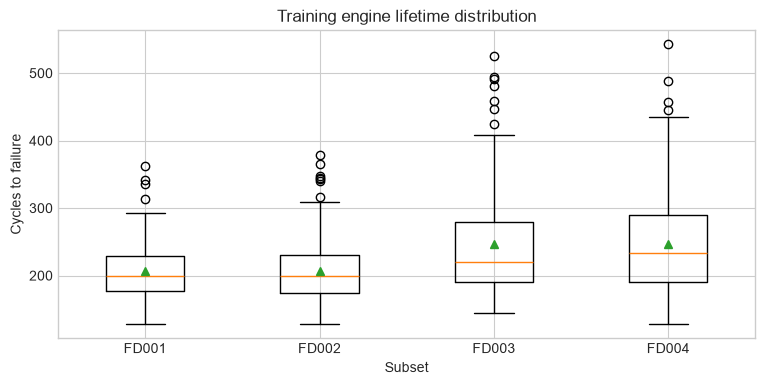
\includegraphics[width=\columnwidth]{../../results/figures/eda_lifetimes.png}
\caption{Distribution of training-engine lifetimes per subset. Triangles mark
the mean.}
\label{fig:eda_lifetimes}
\end{figure}

\subsubsection{Some sensors carry no information in FD001}
Six FD001 sensors are exactly constant across all training rows: $s_1$, $s_5$,
$s_{10}$, $s_{16}$, $s_{18}$ and $s_{19}$. They cannot separate healthy from
degraded engines, so the default selection rule removes them. Three further
channels, $s_6$, $s_8$ and $s_{13}$, vary very little relative to their mean,
but small variation is not the same as no information, and they are retained.
FD003 has five constant sensors, and FD002 and FD004 have none, because a
sensor that is fixed within one operating condition still changes between
conditions.

\subsubsection{Operating conditions dominate raw sensor levels}
The operating settings of FD002 and FD004 fall into six tight clusters
(Fig.~\ref{fig:eda_opsettings}), matching the six simulated flight conditions.
Fig.~\ref{fig:eda_hist} shows the consequence. In FD001 each sensor has a
single, roughly bell-shaped distribution, whereas in FD002 the same sensors
split into separate modes, one or more per condition, spread over a range much
wider than the change caused by degradation. Pooled statistics such as
correlations are therefore confounded by the operating condition in these
subsets. This finding motivates normalizing each sensor within its learned
operating regime before computing degradation features.

\begin{figure}[!t]
\centering
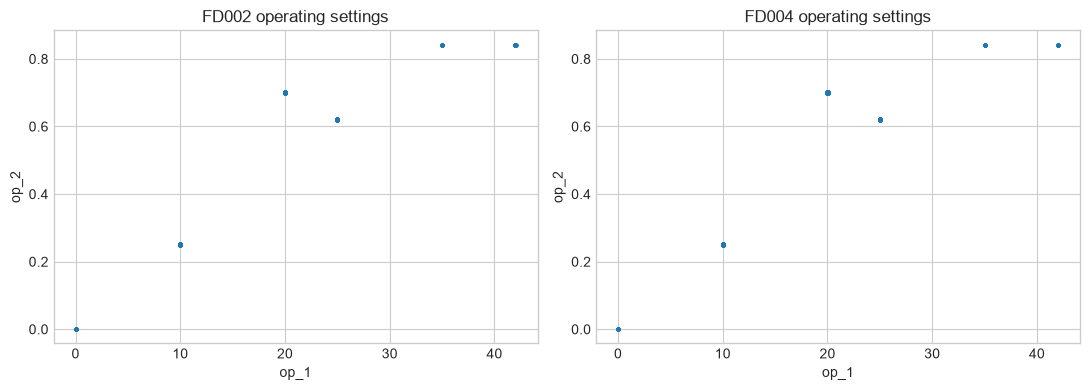
\includegraphics[width=\columnwidth]{../../results/figures/eda_op_settings.png}
\caption{Operating settings \texttt{op\_1} and \texttt{op\_2} for FD002 and FD004
training rows (10,000-row random samples). Each cluster is one operating
condition.}
\label{fig:eda_opsettings}
\end{figure}

\begin{figure*}[!t]
\centering
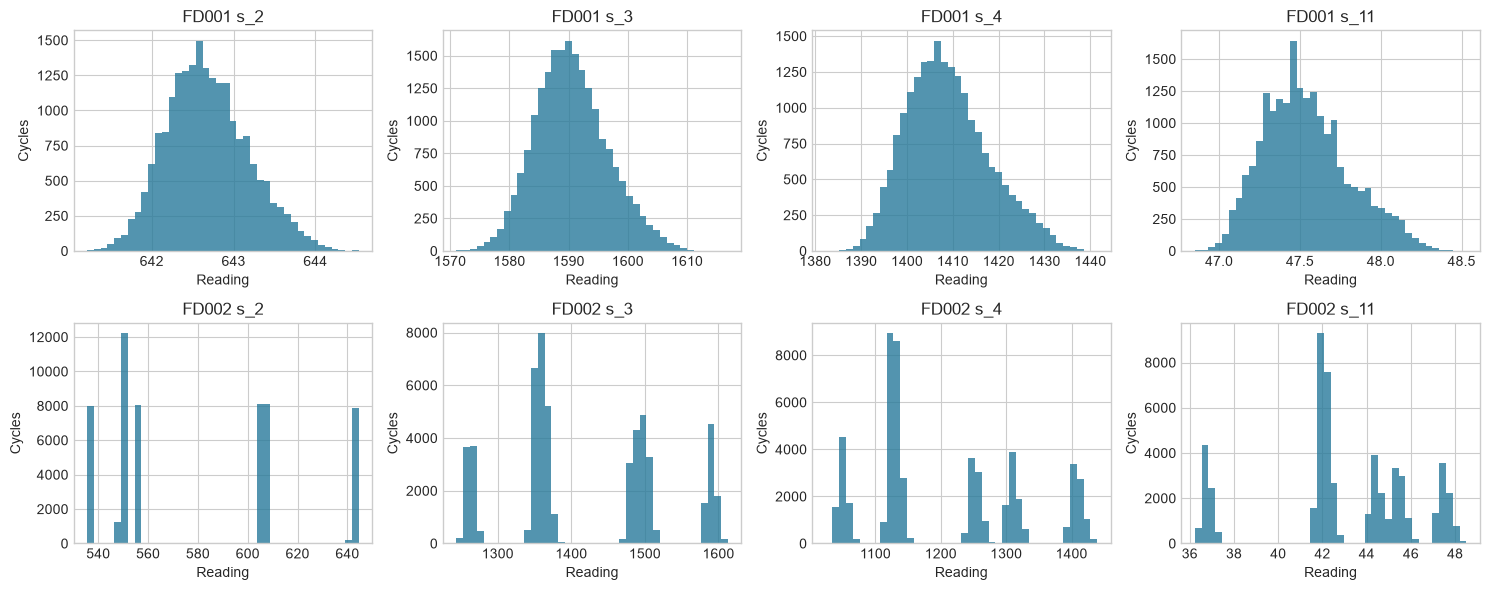
\includegraphics[width=\textwidth]{../../results/figures/eda_sensor_hist.png}
\caption{Raw readings of four sensors over all training cycles in FD001 (top,
one operating condition) and FD002 (bottom, six operating conditions).}
\label{fig:eda_hist}
\end{figure*}

\subsubsection{Degradation is slow early and accelerates near failure}
To compare engines of different lengths, Fig.~\ref{fig:eda_trends} averages
FD001 sensor readings in bins of the fraction of each engine's observed life.
The informative sensors $s_2$, $s_3$, $s_4$ and $s_{11}$ change little during
roughly the first half of life and then rise increasingly steeply until failure.
This shape is consistent with the exponential fault growth of the simulation
model~\cite{Saxena2008damage}. It has two implications. First, the level and
the recent slope of a sensor both carry information, which motivates the
rolling mean and slope features. Second, early-life cycles look alike in the
sensors while their true RUL differs widely, so errors on early cycles are
expected to be large under the uncapped target; this is why errors are broken
down by degradation stage and a capped target is checked as an ablation
(Section~\ref{sec:results}). The
life fraction uses each training engine's final cycle and is used here only
for description; it is never a model input. Individual engines are noisier
than these averages, and they start from different levels because initial
wear differs.

\begin{figure*}[!t]
\centering
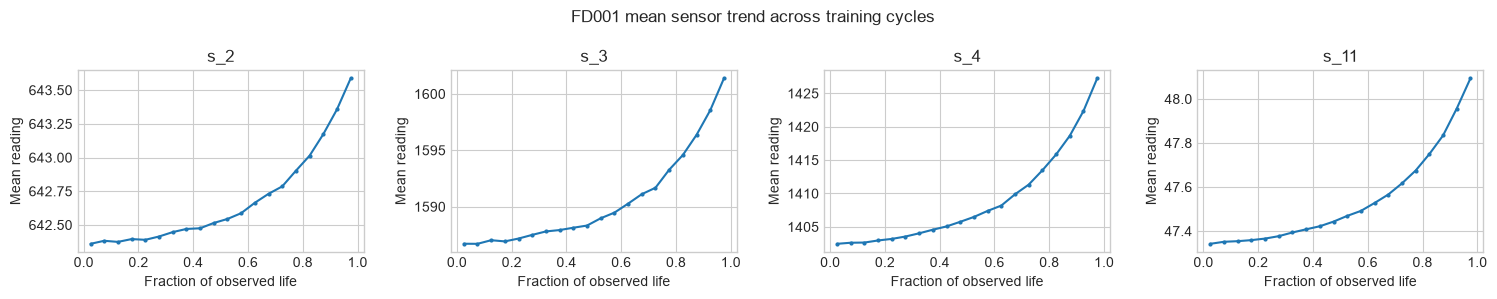
\includegraphics[width=\textwidth]{../../results/figures/eda_fd001_sensor_trends.png}
\caption{Mean FD001 training reading of four sensors in 20 bins of the fraction
of each engine's observed life.}
\label{fig:eda_trends}
\end{figure*}
